\documentclass{article}
\usepackage{../../../LaTeX-Preamables/Base}

\begin{document}


\section*{Data warehousing}

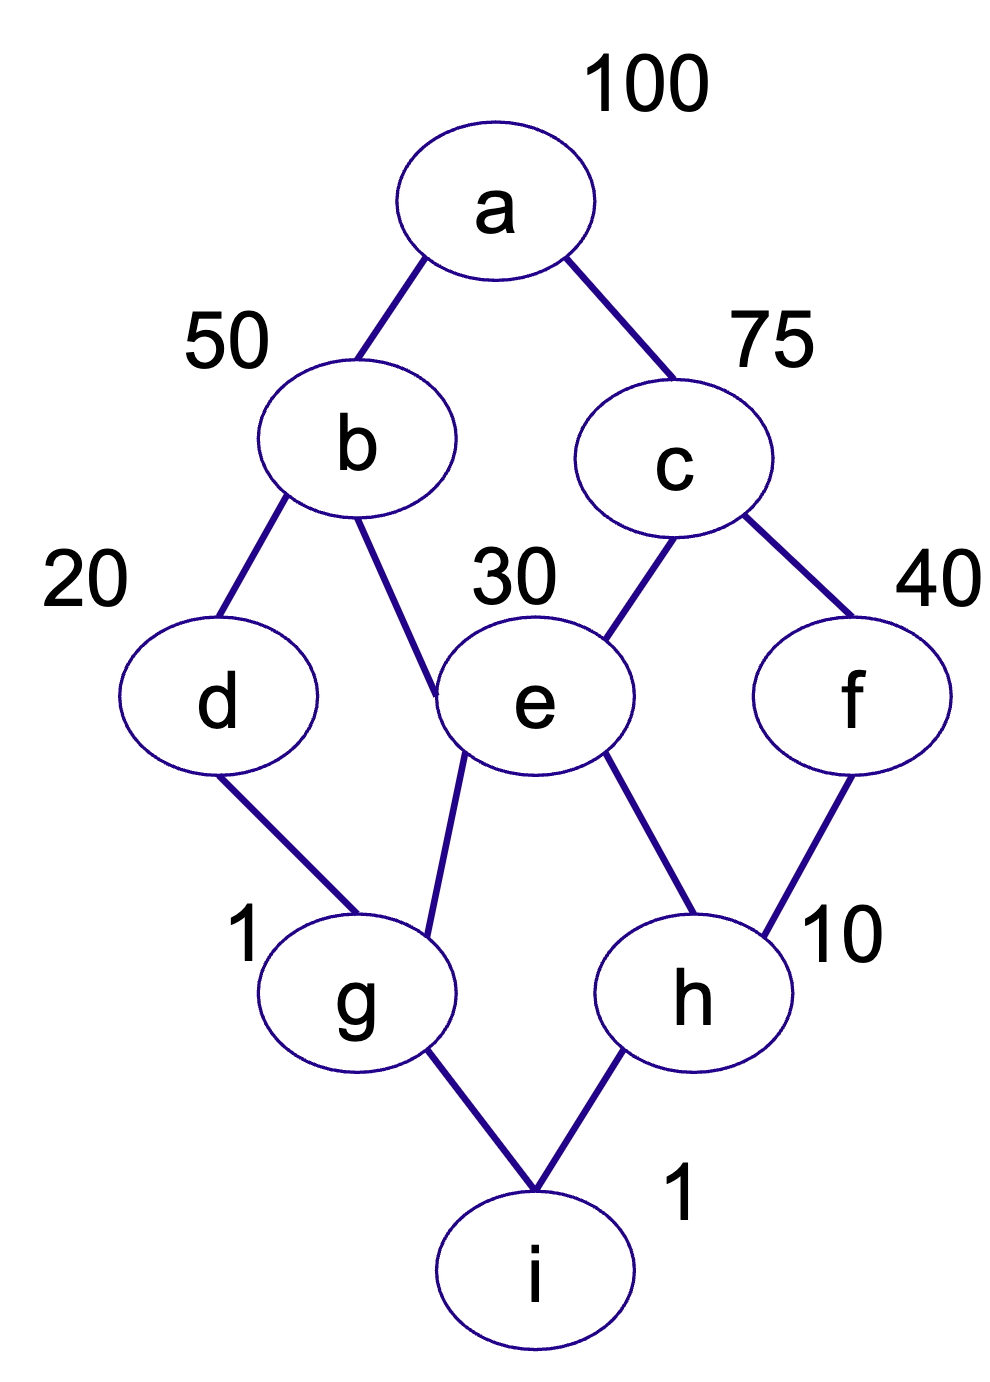
\includegraphics[width=.1\textwidth]{datawarehouse.png}

% Two dimension heirarchies:
% \begin{itemize}
%     \item a 100
%     \item b 50, c 75
%     \item d 20 e 30 f 40
%     \item g 1 h 10
%     \item i 1
% \end{itemize}

Assume a is already materialized.

% Benefit(view) = (size(closest_materialized_ancestor) − size(view)) × (# of nodes in view’s subtree including itself)

\begin{tabular}{l|l}
    View & 1st choice benefit with $v=a$ \\
    \hline
    b    & $(100-50) \times 6 = 300$     \\
    c    & $(100-75) \times 6 = 150$     \\
    d    & $(100-20) \times 3 = 240$     \\
    e    & $(100-30) \times 4 = 280$     \\
    f    & $(100-40) \times 3 = 180$     \\
    g    & $(100-1) \times 2 = 198$      \\
    h    & $(100-10) \times 2 = 180$     \\
    i    & $(100-1) \times 1 = 99$       \\
\end{tabular}

Largest benefit: b (300)

\textbf{$\to$ Materialize b}.

\begin{tabular}{l|l}
    View & 2nd choice benefit with $v=$ \\
    \hline
    c    & $(100-75) \times 2= 50$      \\
    d    & $(50-20) \times 3= 90$       \\
    e    & $(50-30) \times 4= 80$       \\
    f    & $(100-40) \times 1= 60$      \\
    g    & $(50-1) \times 2= 98$        \\
    h    & $(50-10) \times 2= 80$       \\
    i    & $(50-1) \times 1= 49$        \\
\end{tabular}

Largest benefit: g (98)

\textbf{$\to$ Materialize g}.

\begin{tabular}{l|l}
    View & 3rd choice benefit with $v=g$ \\
    \hline
    c    & $ (100-75)\times 2 = 50 $     \\
    d    & $ (50-20)\times 1 = 30 $      \\
    e    & $ (50-30)\times 2 = 40 $      \\
    f    & $ (100-40)\times 1 = 60 $     \\
    h    & $ (50-10)\times 1 = 40 $      \\
    i    & $ (1-1)\times 1 = 0 $         \\
\end{tabular}

Largest benefit: f (60)

\textbf{$\to$ Materialize f}.

\textbf{Answer: Materialize views b, g, f.}

\end{document}